\documentclass[11pt]{scrartcl}
\usepackage[top=1cm, bottom=2.5cm, left=2.5cm, right=2.5cm]{geometry}
\usepackage{graphicx,float}
\usepackage{url}
\usepackage[T1]{fontenc}
\usepackage[font=small,labelfont=bf,tableposition=top]{caption}
\usepackage{amsmath,amssymb,amsfonts}
%\usepackage{algorithm, algorithmic}
%opening
\usepackage{titling}
\usepackage{multirow}
\setlength{\droptitle}{-2cm}
\title{Project Report 3}
\author{Fuyuan Lyu, Tianyu Shi, Dingyi Zhuang}

\begin{document}

\maketitle

\begin{abstract}
In this project, we build several models to classify image data. We use the CIFAR 10 dataset with the default test and train partitions.
Then we build several models, including Multilayer perceptron, Convolutional Neural Network...(should we add more?). We have done several experiments on preprocessing methods, neural network structure, and parameter tuning.
\end{abstract}
  
\section{Introduction}
The goal of this project is to investigate the performance of different models upon the CIFAR-10 dataset. The CIFAR-10 dataset is a collection of images that are commonly used to train machine learning and computer vision algorithms. The CIFAR-10 dataset contains 60,000 32x32 color images in 10 different classes.The 10 different classes represent airplanes, cars, birds, cats, deer, dogs, frogs, horses, ships, and trucks. There are 6,000 images of each class.

In the pre-processing stage, we have tried several data augmentation techniques, including Using the Random Horizontal Flip, Random Crop Transforms and Normalization on both training and testing set. Data augmentation can make our trained models more robust and capable of achieving higher accuracy without requiring larger dataset.
We have also tried to normalize the image dataset. All values in the image data set originally ranges from 0 to 255. When back-propagation process is performed to optimize the networks, this could lead to an exploding/vanishing gradient problems. In order to avoid the issue, it is better let all the values be around 0 and 1.
Furthermore, we also tried one hot encoding for each labels. A vector having the same number of elements as the number of classes of the image is implemented. For instance, CIFAR-10 provides 10 different classes of the image, so we build a vector in size of 10 as well, which can guarante our models to do a better job in prediction period.



\section{Related Work}
The Image classification task is a classical problem in computer vision field. In this task, models takes the pixel-based images as input and aims to successfully classify it to given labels. When multilayer perceptron is processing such tasks, it vectorize the whole images and ignore the spatial structure of the image. One multilayer perceptron has the characteristic of fully connected layers and consists at least three such layers. The pros is that all neurons have the feedforward information of all neurons from the previous layer, while the cons is that this mechanism may contains too much weights and prone to overfitting.

Later, multilayer perceptron is deemed insufficient for more advanced computer vision tasks and replaced by convolutional neural network\cite{krizhevsky2012imagenet}, which use convolution operation as the basic component, after its success in ImageNet challenge\cite{deng2009imagenet}. Nowadays, the structure of convolution neural network has evolved and changed a lot from the original structure. But in this project, we will stick the classic version.



\section{Dataset preprocessing}
We use the CIFAR-10 dataset to train and test our model. The original one batch data is (10000 x 3072) matrix expressed in numpy array. The number of columns, (10000), indicates the number of sample data. As stated in the CIFAR-10 dataset, the row vector, (3072) represents an color image of 32x32 pixels. 
We reshape and transpose the original input image data in the form of $width \times height \times num_{channel}$ in order to feed it into our models.
We then build the normalization function which takes data, x, and returns it as a normalized Numpy array. In our model, x is a  3-D array for an image. Min-Max Normalization (y = (x-min) / (max-min)) technique is used to transform the original image into the range of 0 to 1. 
Furthermore, we build one hot encode function which takes the input, x, which is a list of labels(ground truth). The total number of element in the list is the total number of samples in a batch. One hot encode function returns a 2 dimensional tensor, where the number of row is the size of the batch, and the number of column is the number of image classes.
Finally, we apply several data autmentation techniques for both training and testing parts. A typical example augmented image sets are shown in figure \ref{data_aug}.

\begin{figure}[H]
	\centering
	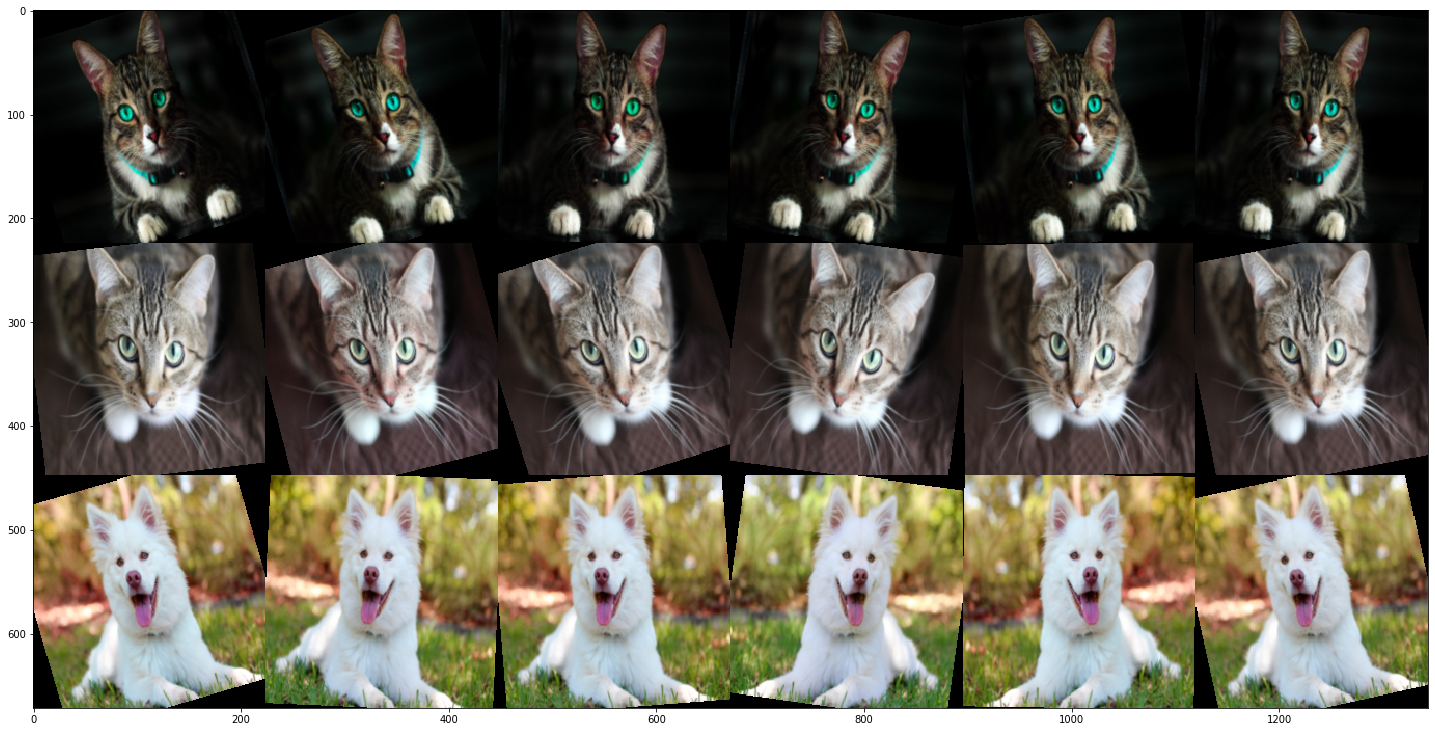
\includegraphics[width=0.9\linewidth]{fig/random_flip_crop_padding.png}
	\caption{Data augmentaion technique based on random flip and crop}
	\label{data_aug}
\end{figure}

\section{Proposed approach}


\section{Results}


\section{Discussion and Conclusion}

\section{Statement for Contributions}
\begin{itemize}
	\item Fuyuan Lyu: 
	\item Tianyu Shi: 
	\item Dingyi Zhuang: 
\end{itemize}
\newpage

\bibliographystyle{unsrt}
\bibliography{ref}

\end{document}
